\documentclass[12pt]{article}

\usepackage{xspace}
\newcommand{\eg}{e.g.\@\xspace}
\newcommand{\ie}{i.e.\@\xspace}
\newcommand{\normal}{\mathcal{N}}
\newcommand{\GEV}{\operatorname{GEV}}
\newcommand{\iid}{i.i.d.\@\xspace}
\makeatletter
\newcommand*{\etc}{%
    \@ifnextchar{.}%
        {etc}%
        {etc.\@\xspace}%
}
\makeatother

\newcommand{\expectation}{\ensuremath{\mathbb{E}}}
\newcommand{\variance}{\ensuremath{\mathbb{V}}}
\newcommand{\probability}{\ensuremath{\mathbb{P}}}
\newcommand{\invlogit}{\ensuremath{\text{logit}^{-1}}}
% Packages With Options
\usepackage[letterpaper, margin=1in]{geometry} % page
\usepackage[english]{babel} % language
\usepackage[utf8]{inputenc} % input
\usepackage[inline]{enumitem} 
\usepackage[section]{placeins} % floats appear in the section they were defined in

% Other Package calls
\usepackage{
  array, % for fixed-width tables
  amssymb, amsmath, % for math
  authblk, % for authors
	booktabs, % for nice tables
  csquotes, % better biblatex
  graphicx, % for figures
  indentfirst, % indent the first line
  physics, % for physics notation
  ragged2e, % for better alignment of text
  siunitx, % for SI notation
  nth, % for 1st, 2nd, 3rd, nth
}

% PACKAGE SETTINGS
\setlength{\RaggedRightParindent}{\parindent} % fix ragged right
\graphicspath{{fig/}{../../fig/}}
\sisetup{round-mode=figures,round-precision=3,scientific-notation=false}
\allowdisplaybreaks{} % let the align environment span multiple pages

% arrays with fixed width
\newcolumntype{L}[1]{>{\raggedright\let\newline \\ \arraybackslash\hspace{0pt}}m{#1}}

\title{Climate Change Adaptation: Uncertainty Associated with Sequential Finite Period Decisions under Nonstationarity}
\author[1,2]{James Doss-Gollin}
\author[1,2]{Upmanu Lall}
\author[1,2]{David Farnham}
\affil[1]{Columbia Water Center, Columbia University}
\affil[2]{Department of Earth and Environmental Engineering, Columbia University}

\usepackage[hidelinks]{hyperref}
\usepackage{cleveref}
\usepackage[
  backend=biber,
  doi=true,
  url=false,
  isbn=false,
  style=authoryear-comp,
  %style=nature,
  natbib=true,
  backref=false,
  maxbibnames=3,
  maxcitenames=2,
  uniquename=false,
  uniquelist=false,
  sorting=ynt
]{biblatex}
\renewcommand{\refname}{References}
\renewbibmacro{in:}{}
\AtEveryBibitem{\clearfield{month}\clearfield{pages}}

\addbibresource{../library.bib}

% -----------------------------------------------------------------------------
% AUTHOR AND TITLE AND TITLEPAGE
% -----------------------------------------------------------------------------

\begin{document}
\maketitle
\RaggedRight{}
\begin{abstract}
  Hydroclimatic systems exhibit organized low-frequency and regime-like variability at multiple time scales, causing the risk associated with climate extremes such as floods and droughts to vary at multiple timescales.
  Despite broad recognition of this nonstationarity, there has been little theoretical development of ideas for the design and operation of infrastructure that simultaneously consider the potential for predictability of secular change and regime behavior or low-frequency variability.
  Consequently, existing theories of flood risk assessment are well-suited to analysis of flood adaptation strategies with fixed project operation period \(M\), but not for analysis of sequential decision strategies.
  In this paper we illustrate some basic considerations of uncertainty and risk analysis associated with the sequential decisions that may need to be made for climate risk adaptation in a nonstationary adaptation.
  We simulate synthetic data and fit the resulting simulations in a Bayesian context using stationary and non-stationary models to show that \(\ldots{}\).
  This is a first conceptual step to the development of a full sequential decision analysis approach under nonstationarity.
\end{abstract}


\section{Introduction}

Hydroclimatic systems vary on many timescales, including regime-like variability and secular variability  \citep{Milly2008,Merz2014,Hurst1951,Sveinsson2005,Hodgkins2017,Matalas2012}.
This multi-scale variability greatly complicates the estimation of future flood sequences, leading to ``low confidence in projections of changes in fluvial floods'' \citep{IPCC2012}.
Yet the same memory and low-frequency variability that complicate projecting flood sequences far into the future may also impart some predictability at short timescales \citep{Jain2001}.
The existence of this information gap suggests that approaches for adapting to hydroclimate risks, such as floods, which have short project operation periods, may be preferential in some cases to large and permanent projects with long project operations.

At present, most approaches to nonstationary flood risk management, or climate change adaptation more broadly, have framed the problem first as one of detecting historical change or modeling future change, and then assessing the implications of this change for future infrastructure.
Though more recent studies have pointed out that the paradigm of requiring proof of the existence of trends before adapting to nonstationarity does not lead to optimal decisionmaking \citep{Vogel2013,Rosner2014}, such discussion has also focused on linear time trends and on choosing whether or not to implement a particular adaptation policy with a fixed planning period.
In contrast, public and private actors seeking to adapt to changing flood or climate risk typically have access to a suite of options including large flood control infrastructure, insurance contracts and other financial instruments, vulnerability reduction (\ie{} disaster response training), and exposure reduction (\ie{} moving infrastructure out of the floodplain).
In this context, understanding under what conditions a large, permanent project or small, easily modified adaptation measure are optimal becomes an important question.

In this paper we provide some initial insight into the bias and uncertainty associated with flood frequency estimation for projects as a function of the project planning period \(M\) and the length of the available data record \(N\).
This project planning period can be interpreted as the design life of a physical structure, or as the contract length of a financial instrument.
Our aim is not to identify the ``best'' model, but rather to build some theory as to how the underlying nature of the natural variability and nonstationarity and the choice of model used to model future flood risk map onto estimation bias and variance in the context of many different \(M\) and \(N\).
This estimation bias and variance may map directly onto the price of an insurance contract\footnote{cite} or the possibility of over/under-design of a flood control structure.
Though we focus on flood risk, this type of analysis may be used for understanding the implications of uncertain projections of the future for climate hazards including drought, hurricane, wind, \etc{}.

\subsection{Physical Reasoning}

In order to make probabilistic predictions of future flooding in a particular location, it is helpful to begin by considering the specific physical mechanisms which may lead to flooding in particular location.

Floods may be associated with a single rainfall event or be composed of a sequence of multiple, distinct events over a week or a season, such that there is pre-conditioning of the land surface soil moisture and natural and man-made stores that leads to a high flooding potential.
In large river basins, Lagrangian tracking studies \citep{Gimeno2010} indicate that river flooding often requires the large-scale transport and convergence of moisture  which are driven by specific large-scale climate mechåanisms \citep{Dacre2014,Gimeno2014,Lu2013,Dirmeyer2010}.\footnote{Farnham et al}
For example, major river floods in the Ohio River Basin (USA) in the 20th century exhibit remarkably consistent continental-scale circulation features in the weeks preceding the flood peak \citep{Nakamura2012,Robertson2015}.
Other case studies of  major floods in the Balkans \citep{Stadtherr2016}, Central Europe \citep{Grams2014}, and Paraguay\footnote{Add my work}, and theoretical analyses \citep{Hoskins2015,Screen2014,Coumou2014}, support the hypothesis that persistent, intense rainfall in a particular place is associated with specific and potentially identifiable climate mechanisms.

At the seasonal and sub-seasonal scales, surface temperature boundary conditions are well known to significantly change the mean, variance, persistence, recurrence and spatial structure of atmospheric circulation patterns, as well as moisture availability.
On longer time scales, changes to the physical processes that govern hydroclimate systems, known generically as nonstationarity \citep{Milly2008} can occur due to climate change, river modification, and land use change \citep{Merz2014}.
Thermodynamic scaling arguments predict an intensified hydrologic cycle under global warming due to the Clausius-Clapeyron scaling of the atmosphere's moisture-holding capacity with temperature \citep[see][]{Muller2011,OGorman2015}.
However, these scaling arguments do not in general hold over land \citep{Byrne2015} and typically describe short-duration rainfall maxima rather than persistent and intense rainfall sequences.
As compared with thermodynamic changes there is less certainty as to how large-scale dynamical circulations may respond to warming signals \citep{Shaw2016,Barnes2015}, as the dynamics governing these mechanisms are highly non-linear \citep{Palmer2013} and in general not well resolved by climate models\footnote{Farnham 2018}.

\subsection{Nonstationary Flood Frequency Analysis\label{sec:ffa}}

Classical methods for design of infrastructure first specify a return period \(T\) (\ie{} 100 years), and then design a project that protects against this \(T\)-year event.
The mathematical problem of interest then becomes estimation of the probability distribution \( f(p_T) \), where \( p_T \) is binary event that the threshold \( Q_T \) is exceeded by the annual-maxiumum flood series \( Q(t) \):
\begin{equation}
  p_T(t) \equiv \probability \qty[ Q(t) \geq Q_T] \qqtext{for} t = \qty[t_0 + 1, \ldots, t_0 + M]
\end{equation}
where \( t_0 \) is the first year forecast and \( M \) is the project operation period.
Averaging over the \(M\)-year period, we can write for convenience
\begin{equation}
  p_T = \frac{1}{M} \sum_{t=1}^{M} p_T(t)
\end{equation}
Although in a stationary setting an unbiased estimator of \( P \qty[ Q(t) \geq Q_T] \) converges asymtotically to \(1 - \frac{1}{T}\), the asymmetric uncertainty distribution of the estimate has also prompted the consideration of the potential for over- or under-design for floods if the conditional mean of the estimated distribution of \( Q_T \) is used for design \citep{Stedinger1997}\footnote{Manu has mentioned a Vogel198x citation but I haven't successfully found it.}.

Under classical assumptions of stationarity, the parameters describing the hydroclimate system are assumed independent of time.
Even when this assumption is satisfied, low-frequency variability can lead to a high probability of surprise, particularly when the length of the record used for estimation \(N\) is short \citep{Jain2001,Matalas2012}.
However, widespread acceptance of nonstationarity as a principle has not led to easily generalizable methodologies for nonstationary flood frequency analysis.

One approach is to extend the purely statistical models currently used in the United States \citep{IACWD1982}.
Like the stationary case, there is no consensus as to the proper statistical distribution to use.
Although Bulletin 17-B \citep{IACWD1982} mandates the use of the log-Pearson type III (LP3) model of annual-maximum floods in the United States, annual-maximum floods are also modeled three-parameter distributions such as the generalized extreme value distribution and two-parameter models such as the lognormal (LN2) \citep{Vogel1996}.
Many studies have extended stationary statistical models to include a time trend on one or more parameters \citep{Obeysekera2014,Vogel2011,Serinaldi2015,Strupczewski2001}, an approach which is conceptually and computationally simple but that lacks physical justification.
Rather than conditioning parameters on time, some recent studies have incorporated a climate index or set of climate indices \(X\) as predictor variables for streamflow \citep{Delgado2014,Silva2016,Sun2014,Griffis2007}\footnote{Farnham et al}.
Other studies have used Markov or mixture models \citep{Waylen1986,Sveinsson2005,Griffis2007}, Bayesian approaches for combining information \citep{Lima2016,Bracken2017}, and other more sophisticated statistical models.

An alternative approach is to use numerical models to represent the physical processes at all scales.
Because models are not able to simultaneously represent scales ranging from global-scale climate phenomena to river hydrology, a ``model chain'' approach is used.
A typical model chain might encompass:
\begin{enumerate*}[label= (\roman*) ]
  \item emission scenario;
  \item general circulation model (GCM);
  \item downscaling;
  \item hydrological catchment model; and
  \item flood frequency analysis.
\end{enumerate*}
Typically bias correction is applied at several or steps of the procedure, which can lead to results which are difficult to interpret in a probabilistic context \citep{Dankers2009,Ott2013,Merz2014,Dittes2017}.

\subsection{Decision Approaches}

Despite the abundance of approaches for estimating future flood hazard, each of which may give different estimates of future flood risk, the ultimate goal of flood frequency analysis is to inform risk management decisions.

Risk-based design methods \citep[RBDM; see][]{Rosner2014} recognize that the appropriate level of design may itself be a decision variable.
\citet{Lall1987} considered the uncertainty in the frequency with which floods may exceed the design level for different values of \(p\) (equivalent to different values of \(T\)), and also for different sample sizes for estimation \(N\) and different project operation periods \(M\).
Some prominent methodologies for risk-based design under nonstationary in the water resources literature include robust decision making (RDM)\footnote{(Lempert et al. 2006; Lempert and Groves 2010; Matrosov et al. 2013)}, scenario-neutral planning\footnote{(Prudhomme et al. 2010)}, infogap analysis\footnote{(Ben-Haim 2006; Korteling et al. 2013)}, and decision scaling\footnote{(Brown et al. 2011, 2012; Moody and Brown 2013; Turner et al. 2014)}.

Alternatively, sequential decision models \citep[see][]{Russell2003,Howard1960} allow decision-makers to optimize not only what action to take, but also when to take it.
Sequential decision models have been used in the hydrological literature for sea wall optimization \citep{Lickley2014}.\footnote{need some citations for sequential decisions}
Given that, low-frequency variability or system memory may lead to less uncertain probabilistic forecasts at short times than long times, models which can capture this uncertainty may be particularly advantageous for sequential models.

There is thus \emph{a critical theoretical need for decision frameworks which can compare projects of different operation period} using an arbitrary choice of model of future flood behavior.
In the following sections we illustrate some basic considerations of uncertainty and risk analysis associated with the sequential decisions that may need to be made for climate risk adaptation in a nonstationary environment.
Understanding the full uncertainty associated with thresholds of interest is relevant to many other climate adaptation problems, including infrastructure design for flood management, because we are faced with the task of estimating the infrastructure's probability of failure \(p_T\) for the next \(M\) years, as well as the uncertainty and bias in this estimate.
This is a first conceptual step to the development of a full sequential decision analysis approach under nonstationarity.
We proceed as follows \(\ldots{}\)

\section{Methods}\label{sec:methods}

We use an idealized model to generate sequences of annual-maximum floods, fit these sequences in a probabilistic framework to three flood models that incorporate time in different ways, and evalaluate the performance of these models for multiple observational record lengths \(N\) and project planning periods \(M\).

\subsection{Generating Synthetic Flood Sequences\label{sec:methods-generating}}

We generate synthetic flood sequences from two different simple conceptual models that represent chaotic dynamics and long memory.

For both cases, the expected value of the annual maximum flood flood follows a log-normal distribution:
\begin{equation} \label{eq:lognormal}
  \log Q(t) \big| \mu(t),\sigma(t) \sim \normal \qty(\mu(t), \sigma(t)).
\end{equation}
where the parameters \( \mu(t), \sigma(t) \) are allowed to vary in time following the two approaches outlined below.
For simplicitiy we assume a constant coefficient of variation:
\begin{equation}
  \sigma(t) = \begin{cases} \alpha \mu(t) & \qqtext{if} \alpha \mu(t) \geq \sigma_\text{min} \\ \sigma_\text{min} & \qqtext{else} \end{cases}
\end{equation}
where \(\sigma_\text{min}\) is a small constant that ensures non-trivial noise in the system.
The two models are summarized in \cref{tab:model-generating}.

Though both approaches used to generate sequences \( \mu(t) \) useh highly simplified models neglecting many important mechanisms, they enable us to generate many synthetic sequences of \(\qty[M + N]\) years which exhibit chaotic but organized quasi-periodic behavior (regime behavior or low-frequency variability) plus a trend term, thereby capturing some essential features of hydrological variability.

In \cref{sec:sequence-realistic} we show sequences of streamflow generated by both models for some choices of parameters and discuss the processes which they can reasonably represent.

\begin{table}[bht]
  \begin{center}
    \begin{tabular}{L{1.0in} L{3.0in} L{1.5in}}
      \toprule
        Model Name & Description & Relevant Section \\
      \midrule
        NINO3 & \(\mu(t)\) proportional to synthetic NINO3 time series & \cref{sec:methods-enso} \\
        Markov & \(\mu(t)\) depends only on sequence of latent states generated by Markov chain & \cref{sec:methods-markov} \\
      \bottomrule
    \end{tabular}
  \end{center}
  \caption{Summary of models used for generating synthetic flood sequences\label{tab:model-generating}}
\end{table}

\subsubsection{Synthetic ENSO Model\label{sec:methods-enso}}

ENSO is the dominant mode of tropical climate variability, impacts flood risk around the world, and varies in a quasi-oscillatory manner with variability on the order of \SIrange{4}{6}{year} modulated by low-frequency oscillation \citep[see][for a comprehensive review]{Sarachik2010}.
A \SI{100000}{year} integration of the Cane-Zebiak model \citep{Zebiak1987} was used to produce a monthly NINO3.4 index with stationary forcing as described in \citet{Ramesh2017}.
A \SI{1000}{year} subset of this data is shown in \cref{fig:enso-ts}.
To create an annual time series, we average the October-December months to create a time series \( x(t) \) where \( t \) is taken in annual steps \(1, \ldots, \num{100000} \).

First a sequence of length \(M+N\) is randomly chosen from the \SI{100000}{year} ENSO sequence.
Next, \(\mu\) is calculated following by
\begin{equation}
  \mu(t) = \mu_0 + \beta x(t) + \gamma \qty(t - t_0)
\end{equation}
where \(\sigma_\text{min}\) is a small constant that ensures non-trivial noise in the system.

\subsubsection{Markov Chain\label{sec:methods-markov}}

To create sequences of floods with strong memory and regime-like behavior, we use a 2-state Markov chain to sample a sequence of states that are used to generate \(\mu(t\).

This Markov chain is given a constant probability of persistence which is the same for both states, such that the transition matrix is
\begin{equation*}
  P = \mqty[\pi & 1-\pi \\ 1-\pi & \pi]
\end{equation*}
This is first used to generate a sequence of states \(S(t)\).
The value \( \mu(t) \) depends only on the \(S(t)\) and the time itself:
\begin{equation*}
  \mu(t) = \begin{cases}
    \mu_{0,1} + \gamma_1 \qty(t - t_0) & \qqtext{if} S(t) = 1 \\
    \mu_{0,2} + \gamma_2 \qty(t - t_0) & \qqtext{if} S(t) = 2
  \end{cases}
\end{equation*}
For simplicity, we assume that the coefficient of variation \( \alpha \) is the same for both states.
We also assume \( \mu_{0, 1} \gg \mu_{0, 2} \) so that state 1 can be interpreted as the ``wet'' state and state 2 as the ``dry'' state.

\subsection{Estimating Future Streamflow Sequences\label{sec:estimation}}

We do not, in general, know the true distribution of annual-maximum floods, and as discussed in \cref{sec:ffa} a plethora of approaches have been suggested in the literature.
This paper does not propose new models or suggest a general ``best'' model; instead it aims to describe the total uncertainty in estimates using easily methods which have been well studied in the literature.

In general, each historical \(N\)-year sequence of streamflow is fit to a statistical model, from which 1000\footnote{Check this parameter} sequences of future streamflow are generated using Monte Carlo simulation.
These estimates are then used to calculate \( \hat{p_T} \), and the estimates are evaluated as described in \cref{sec:methods-uncertainty}.
Three models are assessed for estimating future streamflow; they are summarized in \cref{tab:model-fitting} and described in greater detail below.

\begin{table}[bht]
  \begin{center}
    \begin{tabular}{L{1.25in} L{3.0in} L{1.25in}}
      \toprule
        Model Name & Description & Relevant Section \\
      \midrule
        \texttt{ln2\_stationary} & \( \log Q \sim N \qty(\mu, \sigma) \) & \cref{sec:method-stationary} \\
        \texttt{ln2\_trend} & \(\log Q \sim N \qty(\mu_0 + \beta_\mu \qty[t - t_0], \sigma_0 + \beta_\sigma \qty[t - t_0] ) \) & \cref{sec:method-trend} \\
        \texttt{HMM} & Hidden Markov Model & \cref{sec:method-HMM} \\
      \bottomrule
    \end{tabular}
  \end{center}
  \caption{Summary of models used for fitting\label{tab:model-fitting}}
\end{table}

\subsubsection{Stationary Model\label{sec:method-stationary}}

We do not, in general, know the true distribution of annual-maximum floods, and there has been substantial discussion in the literature as to the choice of distribution to use for stationary flood frequency analysis.
We consider the log-normal model (\cref{eq:lognormal}) for stationary flood distribution; while this model is less flexible than three-parameter models such as the GEV or LP3 \citep{Vogel1996}, it is computationally convenient and easy to understand.
More importantly, since we know the true distribution of these synthetically generated flood, using the log-normal for both generating and fitting supports interpreting results as a lower bound on total uncertainty.
In the stationary context, we assume \(\mu(t) = \mu\) and \(\sigma(t)=\sigma\).

For each simulation, the first \(N\) years \(\qty(t=[t_0-N+1, \ldots, t_0])\) are treated as observations.
Then, once the appropriate time parameterization is selected (\cref{tab:model-fitting}), the parameters are fit in a Bayesian framework to fully represent the posterior uncertainty as implemented in the \texttt{stan} probabilistic programming language \citep{Carpenter2016}.
Weak (uninformative) priors are chosen; in the context of a synthetic data experiment using informative priors seems inappropriate but other studies\footnote{cite} have used scaling information and regional information to inform prior distributions and reduce posterior variance.

\subsubsection{Trend Model\label{sec:method-trend}}

Many studies\footnote{cite} have used time parameterizations for fitting.
We consider a trend model where the data is log-normally distributed as \cref{eq:lognormal} with a linear time trend on both \( \mu \) and \( \sigma \):
\begin{align}
  \mu(t) = \mu_0 + \beta_\mu \qty(t - t_0) \\
  \sigma(t) = \sigma_0 + \beta_\sigma \qty(t - t_0)
\end{align}

As for the stationary case, we fit posterior samples in a Bayesian framework using \texttt{stan} and apply weak priors.
The influence of priors in this case is stronger than in the stationary case, and a reasonable choice of priors might strongly favor \(\beta_mu=0\) and \(\beta_\sigma=0\), for example using the Horseshoe prior parameterization \citep{Piironen2016a}.

\subsubsection{Hidden Markov Model\label{sec:method-HMM}}

A Hidden Markov Model (HMM) is a statistical Markov model in which the system being modeled is assumed to be a Markov process with unobserved (\ie{} hidden) states \citep{Rabiner1986}.
The (unobserved) states evolve following a first-order Markov process, and the observed variable (\ie{} streamflow) depends only on the observed state.
As such, HMMs are a structured prediction method which extend general mixture models to sequences of data, where position in the sequence is relevant.
Because this structure allows the hidden state to represent hydroclimatological ``regimes'' \citep{Reinhold1982,Michelangeli1995,Merz2014}, HMMs have have been used extensively to model hydrological variables such as streamflow \citep{Bracken2016}.
HMMs have also been used to model the evolution of climate states such as ENSO.\footnote{Julian's work}

To supplement the distributional models described in \cref{sec:estimation}, we also fit observed streamflow sequences using a HMM as implemented in the python \texttt{pomegranate} package \citep{Schreiber2016}.
The model is fit to the \(N\) observed years of data using the Baum-Welch algorithm, assuming that the data follow a log-normal distribution conditional only on the state.
To choose the number of hidden states, a log probability score is used.
Future floods are estimated by simulating future states from the resulting matrix and then drawing floods log-normally using the estimated parameters.

\texttt{How much more do we need to say about HMM?}

\subsection{Evaluating Fitting Models}

For a given choice of \(M\), \(N\), generating model, and fitting model, \(J\) sequences of streamflow of length \(M+N\) years each are generated.
For each of the \(J\) sequences, the fitting model is then fit on the \(N\)-year historical record.
\(K\) posterior simulations of future rainfall are then drawn from the fitted model.
We then perform a standard decomposition of uncertainty:
\begin{equation}
  \mathbb{E} \qty[ \qty( \hat{p}_T - p_T )^2 ] = \qty( \mathbb{E} \qty[ \hat{p}_T ] - p_T )^2 + \mathbb{E} \qty[ \qty( \hat{p}_T - \mathbb{E} \qty[ \hat{p}_T ] )^2]
\end{equation}
where the first term is the mean squared error, the second term is the bias squared, and the third term is the variance.

\subsection{Reproducability}

All computation was carried out in the \texttt{python} environment, making particular use of the \texttt{xarray}, \texttt{numpy}, \texttt{pandas}, and \texttt{matplotlib} libraries \citep{Hoyer2017,vanderWalt2011,McKinney2010,Hunter2007}.
To carry implement the flood sequence generating and estimating functions, a new package called \texttt{floodsampling} was developed and is available at \url{github.com/jdossgollin/floodsampling}.
The codes used to generate the figures and text of this paper are available at \url{github.com/jdossgollin/MNpaper}.

\section{Results}

We begin by showing the types of synthetic streamflow sequence that are by the two models discussed \cref{sec:methods-generating}.
We then examine how different statistical models for estimating future flood sequences perform under stationary conditions and when a secular trend is introduced.

\subsection{Are Generated Sequences Realistic?\label{sec:sequence-realistic}}

The models used to generate synthetic flood sequences used simplistic dynamics, but nevertheless were designed to incorporate regime-like and quasi-period variability at multiple timescales.

To verify that these synthetic streamflow sequences sufficiently represent these behaviors, we plot several sequences.
The ENSO model used a long run of the Cane-Zebiak model \citep{Zebiak1987,Ramesh2017} to determine \(\mu(t)\); a \SI{2500}{year} sub-set of the annualized time series is shown in \cref{fig:enso-ts}.
As described in the literature,\footnote{citations, and maybe some paleo stuff as well} this model shows quasi-periodic oscillations in the \SIrange{3}{7}{year} band but with substantial low-frequency modulation of extreme activity.
The index is also asymmetrically distributed, with a longer tail on the positive (El Ni\~{n}o) side than the negative (La Ni\~{n}a) phase, which is consistent with observations of ENSO.

\Cref{fig:stationary-sequences} shows 50 streamflow sequences generated with \(M=50\) and \(N=100\).
The ENSO sequences were generated with \(\gamma=0, \beta_\mu=0.5, \mu_0=6\), which gives a strong (but still noisy) relationship between the NINO3 index \(x(t)\)) and the annual-maximum streamflow \(Q(t)\).
The Markov sequences were generated with \(\mu_1 = 6.55, \mu_2=5.7, \gamma_1=0, \gamma_2=0, \pi=0.9\), which gives a large difference between the two states.
For both, the coefficient of variation \(\alpha=0.1\) and the minimum value of sigma \(\sigma_\text{min}=0.01\).
As the time series plot shows, both generating models exhit substantial persistence in flood probability from one year to the next, though the ENSO model shows negative autocorrelation at lag 1 while the Markov model has positive autocorrelation at lag 1 (not shown).\footnote{Need to include this?}

\begin{figure}[b]
  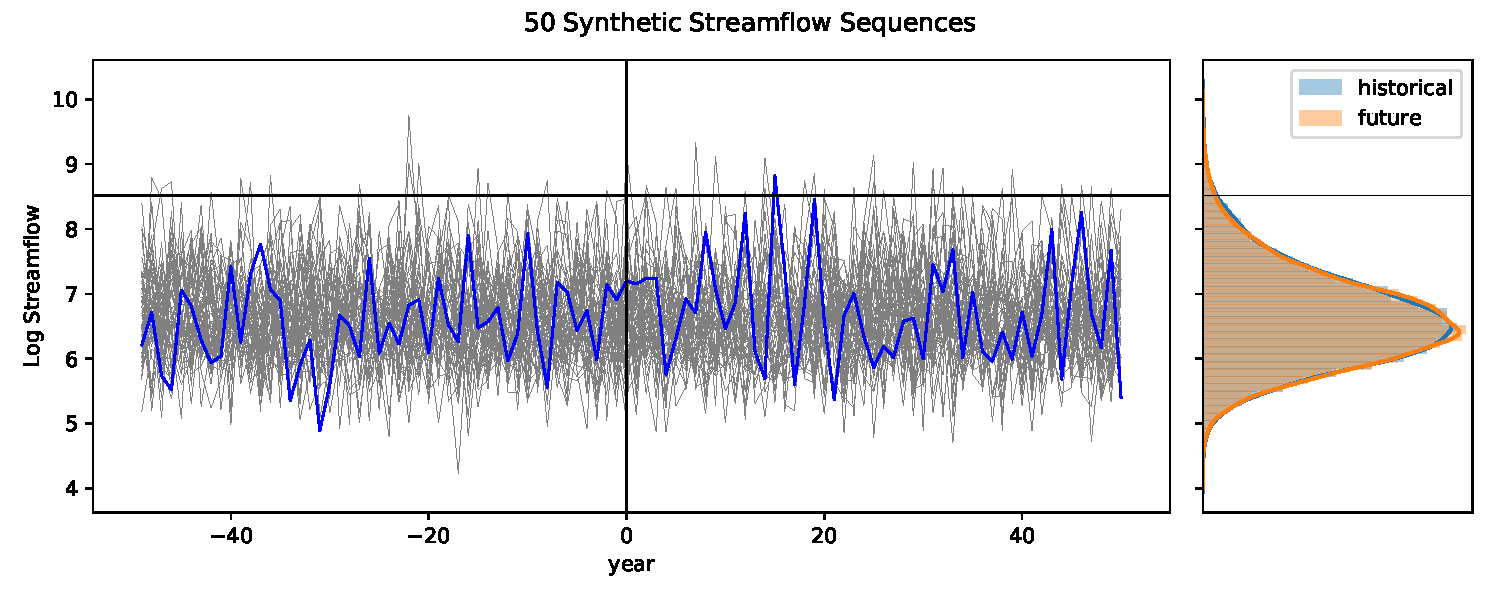
\includegraphics[width=\textwidth]{../../figs/stationary_sequences.pdf}  
  \caption{
    50 streamflow sequences from (Top) the ENSO-based model described in \cref{sec:methods-enso} and (Bottom) the Markov chain modle described in \cref{sec:methods-markov}.
    Both models use a stationary parameterization.
    49 of the 50 sequences are plotted in gray, and one (randomly chosen) is plotted in blue for emphasis.
    The right hand panel shows the distribution over the historical and future periods for 500 sequences from the same model, visualized with a histogram and kernel density estimate.
    Horizontal line shows a threshold of \num{2500}, which is exceeded with probability \num{0.014133333333333333} by the NINO3 sequences and \num{0.013546666666666667} by the Markov sequences.\label{fig:stationary-sequences}
  }
\end{figure}

To incorporate secular variability into our model, we repeat the exercise but add a trend term to the data.
For the ENSO time series, this mean setting \(\gamma=0.02\) while for the Markov case this meant a trend term on the wet state only, so that \(\gamma_1=0.02\).
The resulting sequences are shown in \cref{fig:trend-sequences}.
The trend has an extremely large impact on the probability of an extremely high flood, but the underlying time series structure is generally preserved.
\begin{figure}[b]
  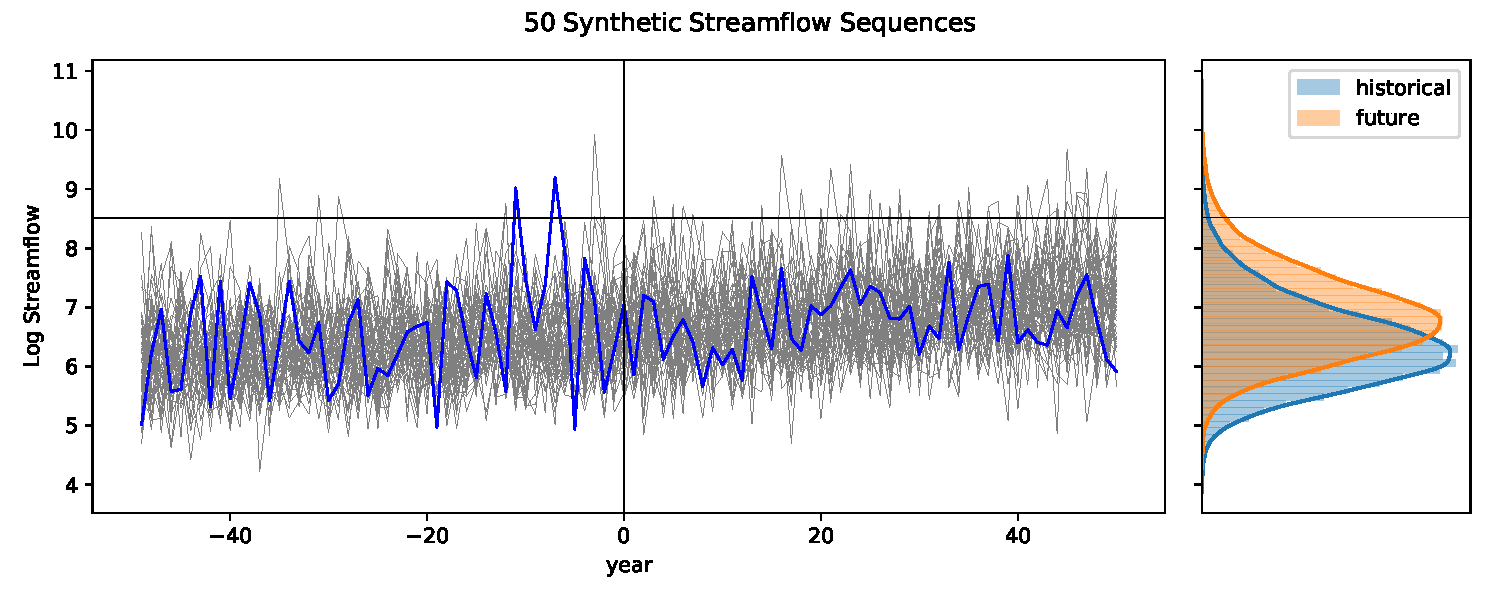
\includegraphics[width=\textwidth]{../../figs/trend_sequences.pdf}
  \caption{
    As \cref{fig:stationary-sequences} but a trend term has been added.
    Horizontal line shows a threshold of \num{2500}, which is exceeded with probability \num{0.023306666666666667} by the NINO3 sequences and \num{0.024493333333333332} by the Markov sequences.\label{fig:trend-sequences}
  }
\end{figure}

\subsection{Stationary Case}

\begin{figure}[ht]
  \includegraphics[width=\textwidth]{../../figs/stationary_bias.pdf}
  \caption{The estimation bias for 1000* sequences generated by each of two stationary generating functions (row) and fit by each of three fitting functions (columns) as a function of \(M\) and \(N\).\label{fig:stationary-bias}}
\end{figure}

\begin{figure}[ht]
  \includegraphics[width=\textwidth]{../../figs/stationary_variance.pdf}
  \caption{The estimation variance for 1000* sequences generated by each of two stationary generating functions (row) and fit by each of three fitting functions (columns) as a function of \(M\) and \(N\).\label{fig:stationary-bias}}
\end{figure}


\subsection{Trend Case}

\begin{figure}[ht]
  \includegraphics[width=\textwidth]{../../figs/trend_bias.pdf}
  \caption{The estimation bias for 1000* sequences generated by each of two non-stationary generating functions (row) and fit by each of three fitting functions (columns) as a function of \(M\) and \(N\).\label{fig:stationary-bias}}
\end{figure}

\begin{figure}[ht]
  \includegraphics[width=\textwidth]{../../figs/trend_variance.pdf}
  \caption{The estimation variance for 1000* sequences generated by each of two non-stationary generating functions (row) and fit by each of three fitting functions (columns) as a function of \(M\) and \(N\).\label{fig:stationary-bias}}
\end{figure}

\section{Case Study}

We still need to find a good case study; it can be a highly simplified one as long as there is a long streamflow record available and building levees is an option that has been proposed.
If there's not an obvious candidate, we can use one of our models above.
We can make some other strong assumptions
\begin{itemize}
  \item Risk exposure constant in time, which allows us to focus on the estimation rather than comprehensive risk manageement
  \item Constant future discounting rate
  \item Flood damages are linearly related to streamflow over some amount:
  \begin{equation}
    \mathcal{D}(t) = k \qty[ Q(t) - Q_T ]
  \end{equation}
\end{itemize}
Then our two options are to build a levee, which we can assume to have a capital cost plus operation and maintenance cost which is proportional to the capital cost, which increases \(Q_T\) by some fixed amount, or to buy insurance.
For the insurance, we consider a contract in which an insurer agrees to pay the entire coverage cost \(C\) every time that the trigger threshold \(Q_T\) is exceeded.
Although \(Q_T\) is in general a decision variable, we treat it as fixed.
Then, using the posterior distribution of the parameters of the chosen statistical model (from \cref{tab:model-fitting}) we estimate the probability that \(Q(t) \geq Q_T\) for \(t \in \vb{t}\), which is equivalent to \(p_T(t)\).
For a particular year, the fair price for the insurance premium is \(\expectation \qty(p_T) C\).
However, there is typically also a risk premium associated with the policy that prices the uncertainty in this estimate (since the trigger \(Q_T\) is specified in the contract and thus not uncertain).
This risk premium is proportional to the variance of \(p_T\), or more generally to its uncertainty distribution.
The insurance premium for a particular year is thus
\begin{equation} \label{eq:premium}
  Z(t) = C \qty[\expectation \qty(p_T(t)) + R \variance \qty(p_T(t))]
\end{equation}
where \(R \geq 0\) is a coefficient describing the cost of tue uncertainty in the estimate of \(p_T(t)\).

Then at each point in time, calculate:
\begin{itemize}
  \item Expected cost plus damage per year for the levee using perfect knowledge of the next 101 years
  \item Expected cost plus damage per year for the levee using MCMC projections of the next 101 years from all 3 models
  \item Expected cost plus damage per year for a 5-year insurance contract using perfect knowledge of the next 5 years
  \item Expected cost plus damage per year for a 5-year insurance contract using MCMC projections of the next 5 years from all 3 models
\end{itemize}

Can add appropriate plot or plots.

\section{Discussion}

For the type of extreme flood events we are interested in, the nominal return period at some location flooded during the event will typically be larger than 10 years.
While this is a relatively rare event at a given location, across a geography as large as the United States, one can expect to see such events rather frequently, emphasizing the need to understand and predict the risk of such events over a season or few years to facilitate preparation and mitigation strategies.

From a decision making perspective, one could either design and build a project that gives us protection through the year 2100 considering both types of nonstationarities, or consider a sequence of projects every M years that incrementally add (or not) protection. How does the uncertainty and hence risk for these decisions manifest depending on the design level p, the duration M, and the uncertainty associated with the estimation of the \( f(Qp(t)) \) given a methodology used for prediction -- \eg{} the model chain using gcms and such and models fitted to a historical data length \(M\).
WHat is the implication for choices of p and M under different models for stationarity and uncertainty using some simple loss and cost  functions.

How could  financial risk mitigation instruments be used in conjunction with structural design to identify a robust, adaptive climate risk mitigation strategy with sequential decisions that are informed by updated estimates of risk.


\section{Summary}

The main point you are hitting is that the very nature of climate has long memory and some people point this out, many model it, and most future projections don't show this.
All corrections (even if we like them) address the marginal distribution.
So while the debate you refer to is interesting to a degree, the point we are making is that in terms of risk analysis it is not even tangentially relevant to reality and what we bring up -- our focus -- is strictly the risk based decision process and we are agnostic to the details of the models, other than the long memory features and spatial teleconnections associated with them that are seen as marks of the system behavior.
We actually demonstrate that the potential loss in a 2100 scenario has to be catastrophic and really out of the range of any historical variability for it to be relevant.
If we accept this proposition then we have a strong case for the mitigation of climate change but a much weaker case for adaptation, since if we are not able to mitigate that scenario then building a giant wall to control the 2100 scenario today will be economically and socially infeasible anyway.
So the next obvious question is in which situation would waiting and updating the decision make sense and this can be set up and explored or just discussed.


% -----------------------------------------------------------------------------
% END HERE
% -----------------------------------------------------------------------------
\appendix
\printbibliography{}

\section{Notation}

\begin{description}
  \item[\( Q(t) \)] Annual-maximum flood series
  \item[\( T \)] Return period, in years
  \item[\( Q_T \)] Flood threshold
  \item[\( M \)] the project planning period
  \item[\( N \)] the length of the observational record, in years
  \item[\( x(t) \)] the annualized time series of the NINO3 index
  \item[\( p_T \)] the true probability that \( Q(t) \geq Q_T \) in the future \(M\)-year period
  \item[\( \hat{p}_T \)] the estimated probability that \( Q(t) \geq Q_T \) in the future \(M\)-year period
\end{description}

\section{Supplemental Figures}

\begin{figure}
  \includegraphics[width=\textwidth]{../../figs/enso.pdf}
  \caption{
    A \SI{2500}{year} sub-set of the synthetic time series described in \cref{sec:methods-enso}.\label{fig:enso-ts}
  }
\end{figure}

\begin{figure}
  \includegraphics[width=\textwidth]{../../figs/example_long.pdf}
  \caption{
    A single sequence of streamflow generated by the NINO3 function with (L) no trend and (R) \(\gamma=0.01\). 
    The sequence is fit to each f`it to three different fitting models (rows). 
    Generated with \(M=N=150\).\label{fig:example-long}
  }
\end{figure}

\begin{figure}
  \includegraphics[width=\textwidth]{../../figs/example_short.pdf}
  \caption{
    As \cref{fig:example-short} except \(N=30\).\label{fig:example-short}
  }
\end{figure}


\end{document}
